\section{Công trình liên quan}

\begin{frame}{Các phương pháp}
\textbf{Rule Base \& Statistic}
\begin{itemize}
	\small
	\item BEAT, Rule-based generation.
	%					 \cite{cassell2001beat}
	\item Gesture Controllers 
\end{itemize}
%	\textit{Nhược điểm}: Không có khả năng mở rộng, kết quả không tốt với các dữ liệu ngoài tập huấn luyện.

\textbf{Deep Learning}
%\begin{itemize}
%	\small
%	\item \textbf{MLP}: Gesticulator
%	\item \textbf{RNN}: Speech2AffectiveGestures, HA2G, TransGesture, .. 
%	\item \textbf{Normalising Flows}: Text2gestures, Speech2Gesture,; \textbf{GAN}: DiffGAN
%	\item \textbf{VAE/VQ-VAE}:  Audio2Gestures; 
%	\item \textbf{Diffusion}: Listen denoise action, DiffuseStyleGesture, Taming Diffusion Models.
%\end{itemize}
\begin{columns}
	\begin{column}{0.5\textwidth}
			{
			\small
			\textbf{Likelihood-based models}:
			\begin{itemize}
				\item \textbf{MLP}: Gesticulator
				\item \textbf{RNN}: Speech2AffectiveGestures, HA2G, TransGesture, .. 
				\item \textbf{Normalising Flows}: Text2gestures, Speech2Gesture
				\textbf{VAE/VQ-VAE}:  Audio2Gestures; 
				\end{itemize}
			}
			 \begin{figure}
				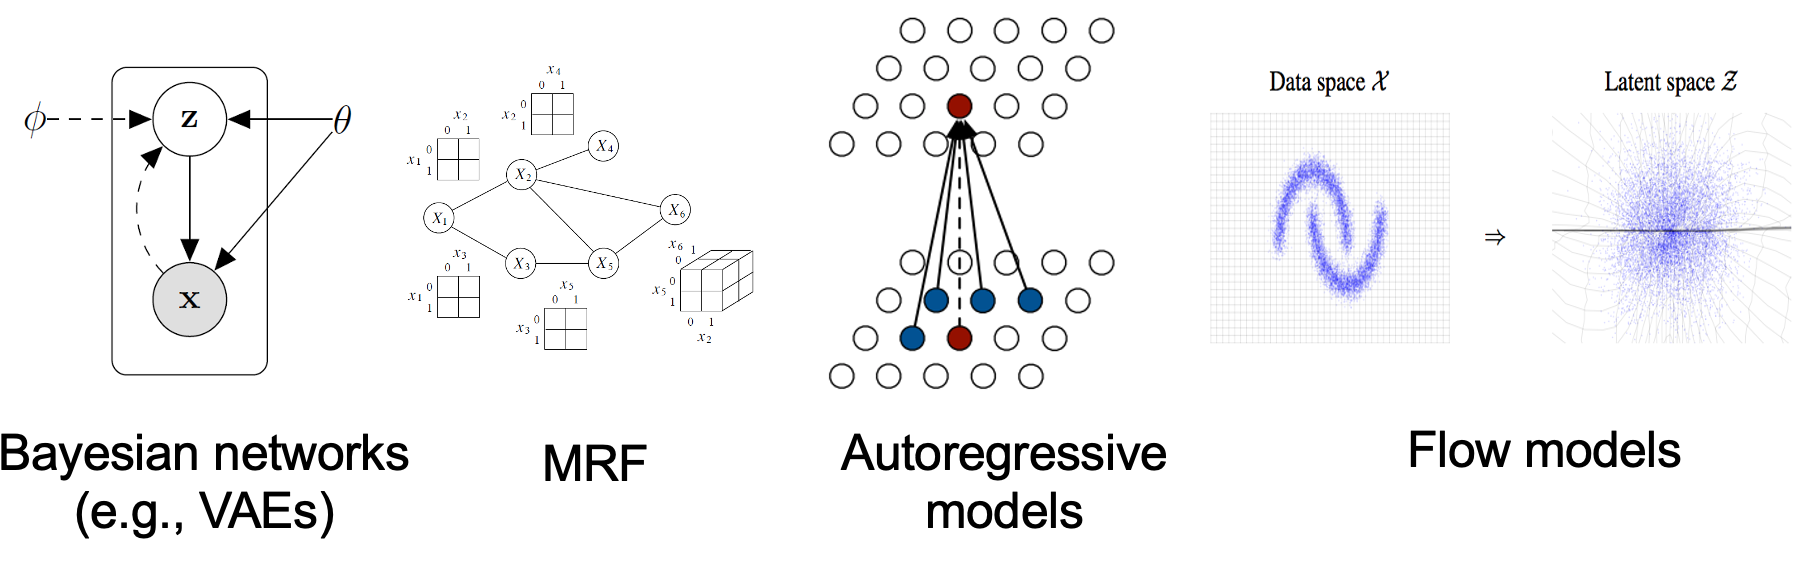
\includegraphics[width=\textwidth]{likelihood_based_models}
			\end{figure}
	\end{column}
	\hspace{-20pt}
	\begin{column}{0.5\textwidth}
		{
			\small
			\textbf{Implicit generative models}:
\begin{itemize}
			\item \textbf{GAN}: DiffGAN
			
			\item \textbf{Diffusion}: Listen denoise action, DiffuseStyleGesture, Taming Diffusion Models.
 \end{itemize}
 
 \begin{figure}
 	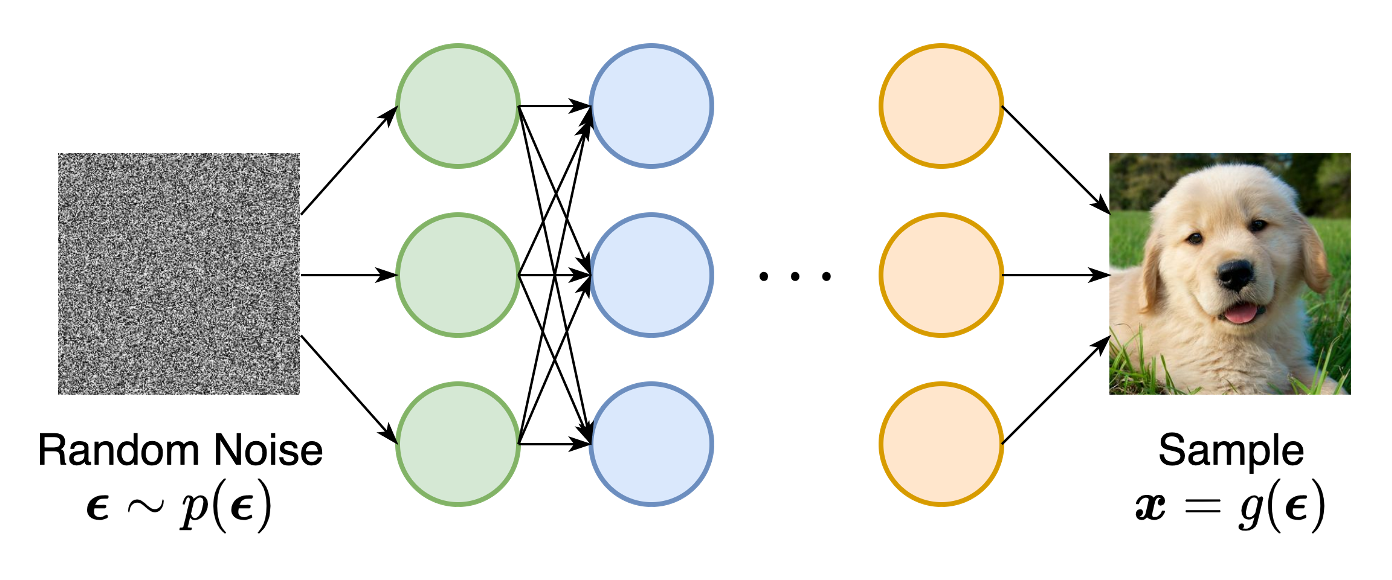
\includegraphics[width=\textwidth]{implicit_models}
 \end{figure}
 
		}
	\end{column}
\end{columns}

%	\textbf{Phase Manifold} : 
%	
%	\begin{itemize}
%		\small
%		\item  DeepPhase , Walk the Dog
%	\end{itemize}

	

%\textbf{Baseline}: \textit{Motion Diffusion Model} (MDM)

%\begin{columns}
%\begin{column}{0.55\textwidth}
	
%\end{column}			
% 
%	
%	\begin{column}{0.45\textwidth}
%		
%		\begin{columns}
%			\begin{column}{0.5\textwidth}
%				\begin{figure}
%					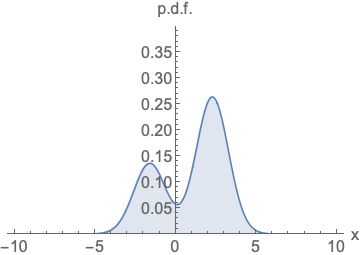
\includegraphics[width=\textwidth]{ProbabilityDensityFunctions.png}
%					\caption{\scriptsize Phải chuẩn hoá (diện tích dưới đường cong phải tích phân thành một)}
%				\end{figure}
%			\end{column}
%			\begin{column}{0.5\textwidth}
%				\begin{figure}
%					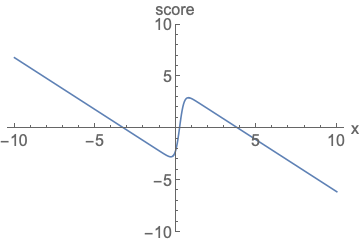
\includegraphics[width=\textwidth]{ScoreFunction.png}
%					\caption{\scriptsize Không cần chuẩn hoá.}
%				\end{figure}
%			\end{column}
%		\end{columns}
%	
%		\begin{columns}
%			\begin{column}{0.5\textwidth}
%				\centering
%				\begin{tikzpicture}
%					\node at (0, 1) {$p(\mathbf{x})$};
%					
%					\node at (0, 0.5) {\small \text{probability density}};
%					
%					\draw[<->, thick] (0, 0) -- (0, -0.5);
%					
%					\node at (0, -1) {$\nabla_\mathbf{x} \log p(\mathbf{x})$};
%					
%					\node at (0, -1.5) {\small \text{score function}};
%				\end{tikzpicture}
%				
%			\end{column}
%			\begin{column}{0.5\textwidth}
%				\begin{figure}
%					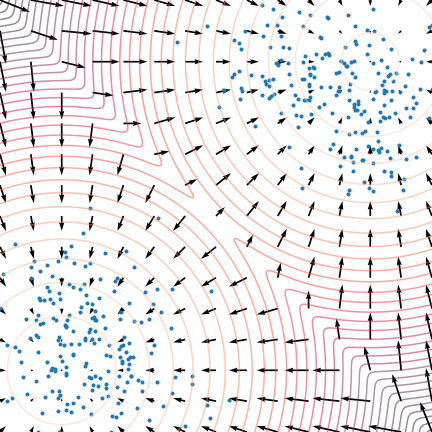
\includegraphics[width=\textwidth]{CompareScoreFunction.png}
%					\caption{\scriptsize score function vs probability density}
%				\end{figure}
%			\end{column}
%		\end{columns}
%	\end{column}
%\end{columns}

%\includegraphics[width=\linewidth]{../animation/ScoreFunction/ScoreFunction\_001}
	
\end{frame}



\begin{frame}{Tư tưởng cơ bản của Diffusion}
	Dataset $\mathcal{G} = \{ x_{i}^{M \times D} \}_{1}^{n}$, ta chuẩn hoá dữ liệu $\bx_{i}^{M \times D} = \frac{\bx_{i}^{M \times D} - \mu}{\sigma}$
\begin{figure}
	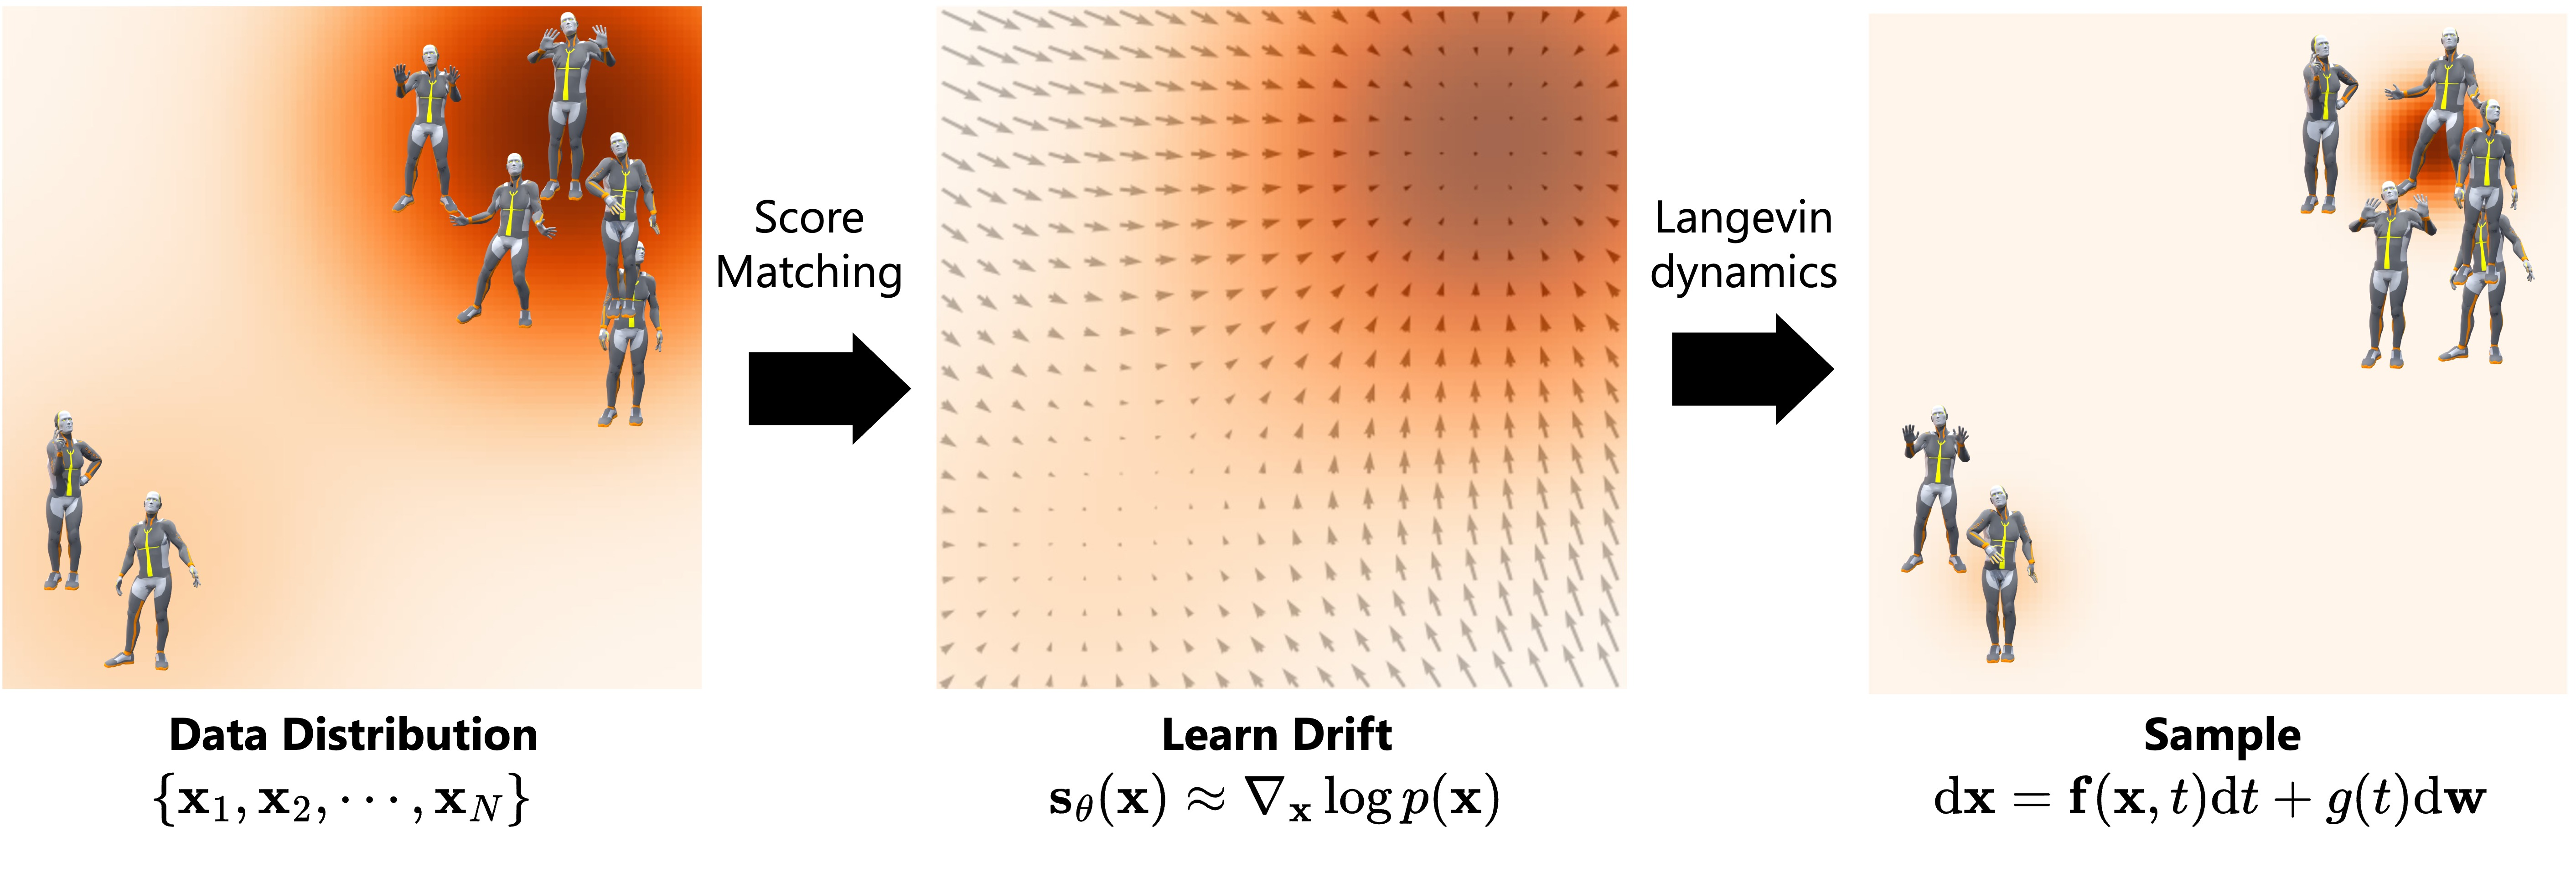
\includegraphics[width=0.8\textwidth]{ScoreMatching}
\end{figure}
\vspace{-10pt}
\begin{figure}
	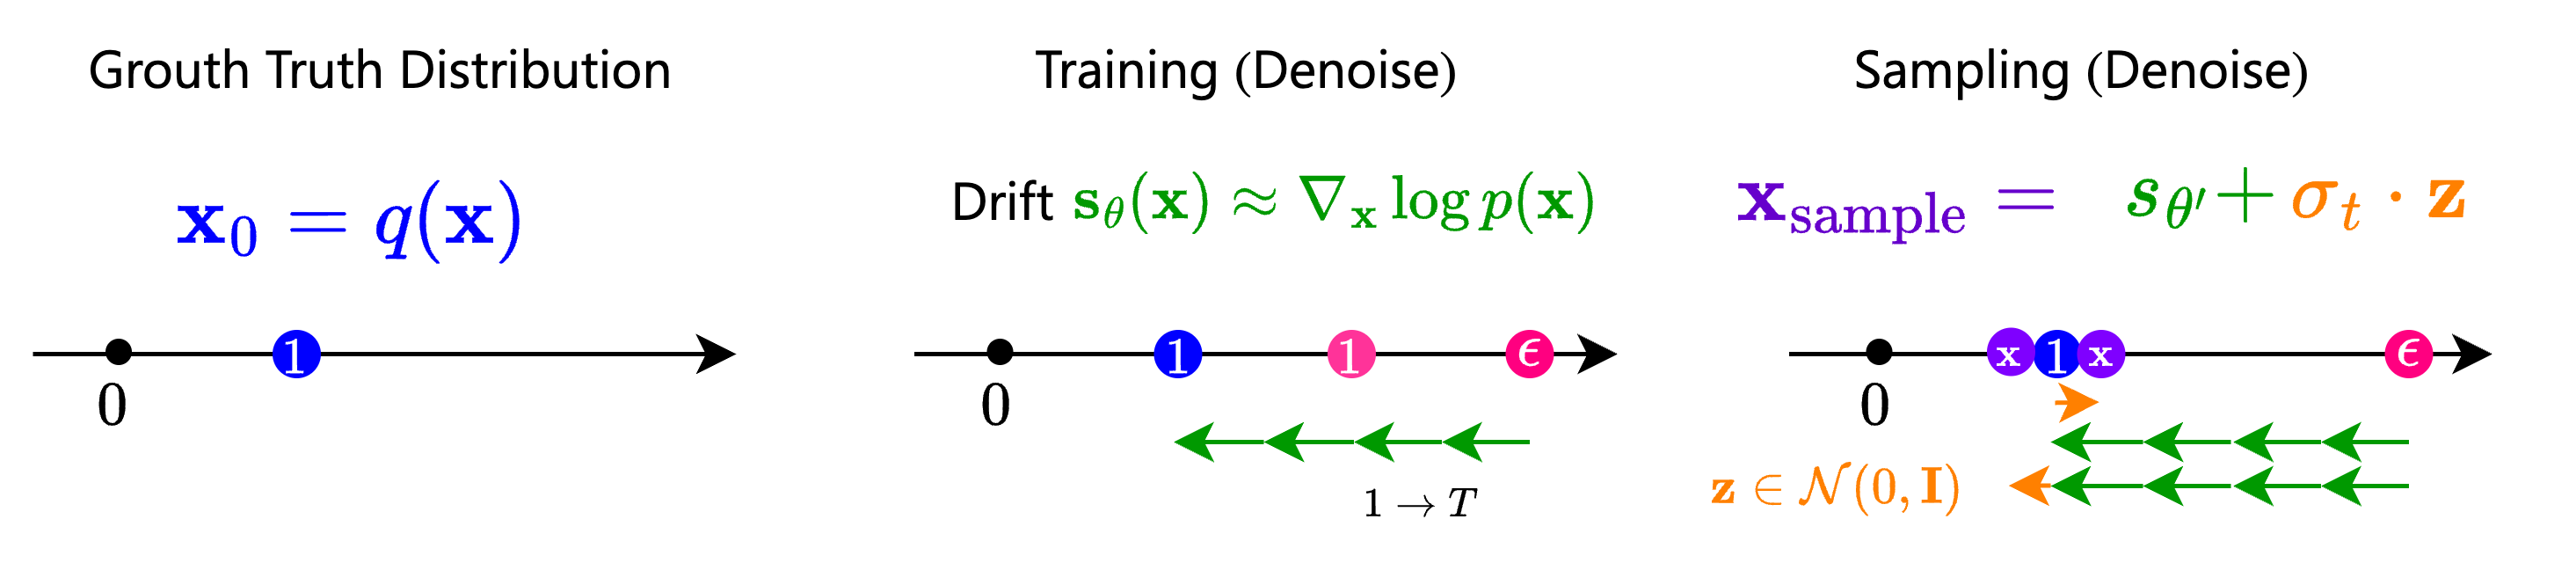
\includegraphics[width=\textwidth]{ScoreDrift}
\end{figure}

\vspace{-10pt}

\begin{figure}
	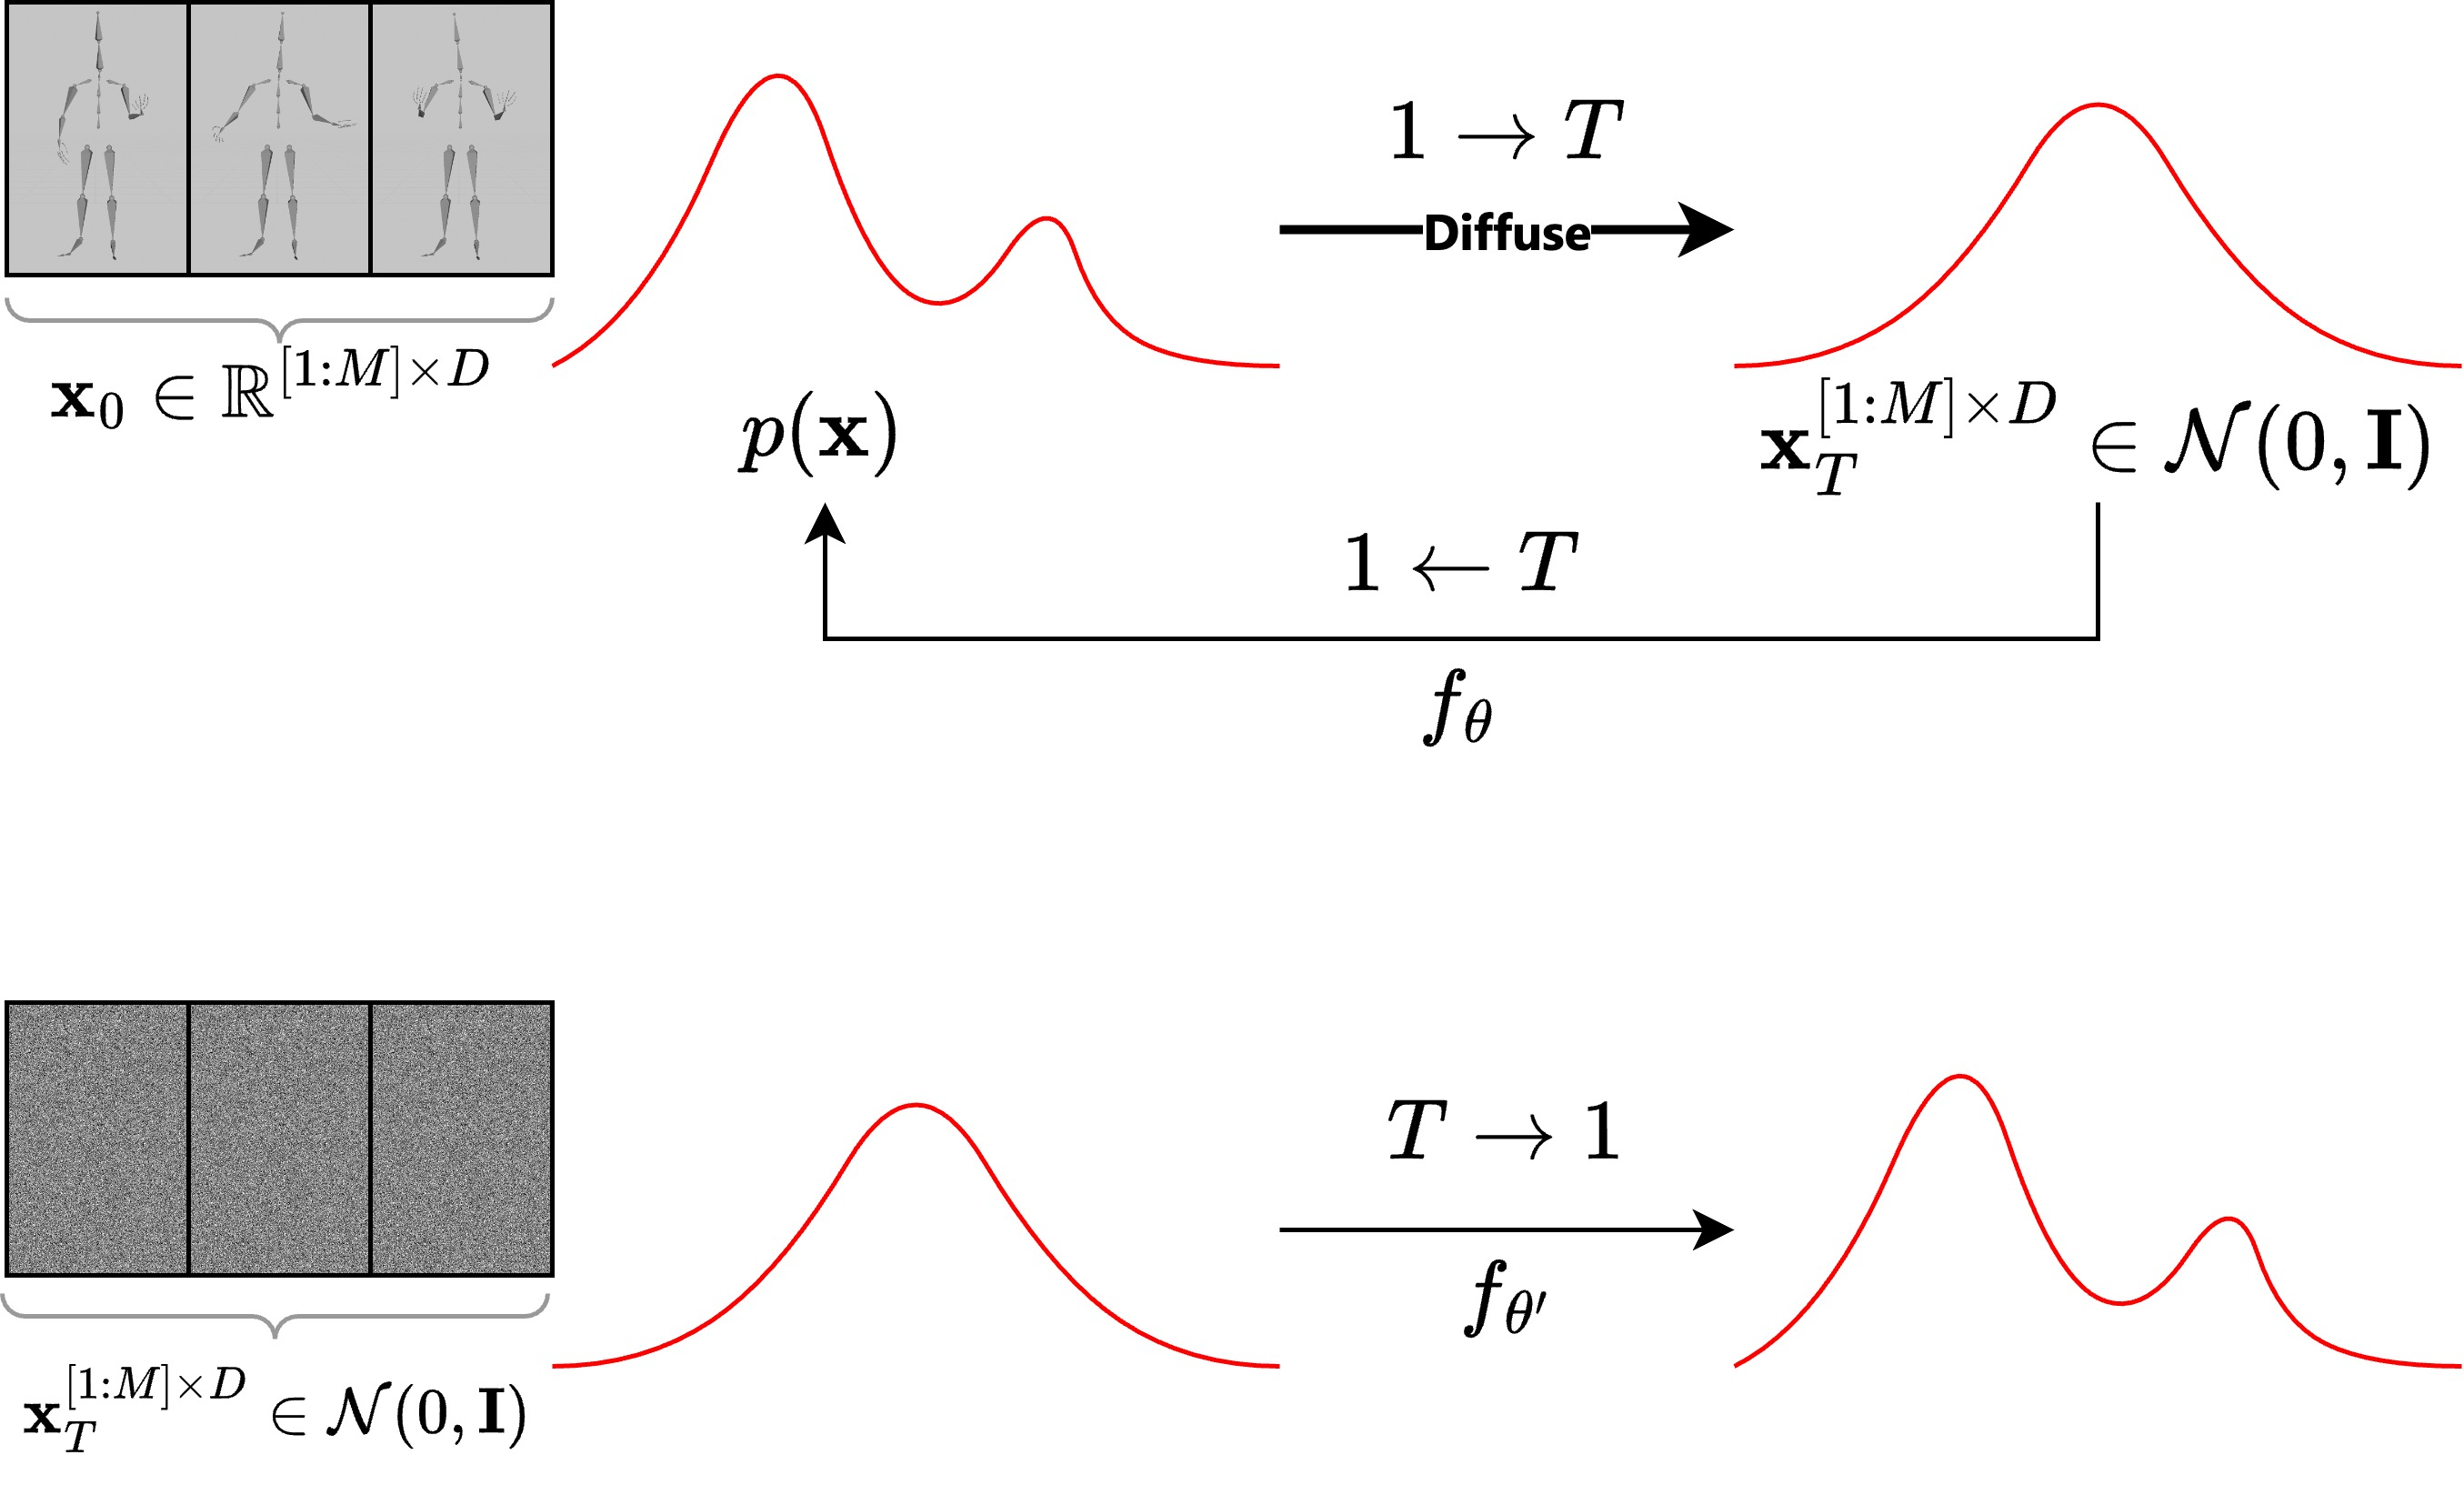
\includegraphics[width=0.8\textwidth]{DistributionTransition}
\end{figure}

\end{frame}

\begin{frame}{Ký hiệu}
	\textbf{Tham số}: Đang huấn luyện {\Large$\textcolor{cyan}{\theta}$}, đã huấn luyện xong: {\Large$\textcolor{cyan}{\theta}'$}, {\Large$\textcolor{cyan}{\hat{\bx}}$}: dự đoán
	\vspace{-5pt}
	
	\textbf{Phân phối chuẩn}
	\vspace{-5pt}
	{\Large $$\mathcal{N}(\textcolor{red}{a} \mathbf{x}, \textcolor{blue}{b^2})$$}
	\vspace{-15pt}
	\begin{itemize}
		\item Một hàm $f(x) = a x + b\epsilon$ với $\epsilon \in \mathcal{N}(0, \mathbf{1})$ được ký hiệu là $f(x) \sim \mathcal{N}(a x, b^2) $
		
		\item Trung bình: $\mu = \textcolor{red}{a}x=\frac{1}{n} \sum_{i=1}^{n} x_i$
		
		\item Phương sai: $\sigma^2 = \textcolor{blue} {b^2} = \frac{1}{n} \sum_{i=1}^{n} (x_i - \mu)^2$
		
	\end{itemize}
	\textbf{Xác xuất có điều kiện}
	\vspace{-5pt}
	{\Large $$p(\textcolor{green}{x}| \textcolor{orange}{y})$$}
	\vspace{-15pt}
	
	\begin{itemize}
		\item $p(\textcolor{green}{x}| \textcolor{orange}{y})$ là xác xuất có điều kiện.
		\item $\textcolor{orange}{y}$: xảy ra trước (bên phải)
		\item $\textcolor{green}{x}$: sảy ra sau y (bên trái)
	\end{itemize}

\end{frame}

\begin{frame}{Đặc điểm của việc học dữ liệu Motion}
	
	\begin{columns}
		\begin{column}{0.55\textwidth}
			\textbf{Quan hệ giữa dữ liệu cử chỉ và âm thanh}:
			\begin{itemize}
				\item Một đoạn cử có thể bao gồm nhiều âm thanh.
				\item Mỗi âm thanh có thể tương ứng với nhiều đoạn cử chỉ khác nhau.
			\end{itemize}
			%		Baseline: \textbf{MDM}  (Human Motion Diffusion Model)
			\textbf{Khó khăn}
			\begin{itemize}
				\item Dữ liệu ít, chi phí cao
				\item Thiếu nhãn và dữ liệu tương ứng giữa âm thanh, cử chỉ.
				\item Quá trình sinh có thể dể điều khiển 
				%			hơn GAN.
			\end{itemize}
			liệu
			%		\textit{Mô hình Diffusion}:
			%		\begin{itemize}
				%			\item Ít yêu cầu về dữ liệu gắn nhãn
				%			\item Khả năng tương tác và điều chỉnh dễ dàng
				%			\item Tính ổn định cao
				%		\end{itemize}
		\end{column}
		\begin{column}{0.45\textwidth}
			
			\begin{columns}
				\begin{column}{0.5\textwidth}
					\begin{figure}
						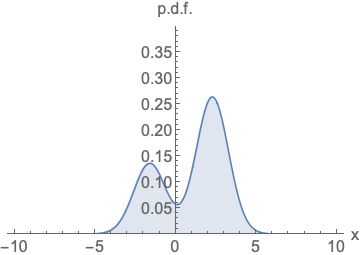
\includegraphics[width=\textwidth]{ProbabilityDensityFunctions.png}
						\caption{\scriptsize Phải chuẩn hoá (diện tích dưới đường cong phải tích phân thành một)}
					\end{figure}
				\end{column}
				\begin{column}{0.5\textwidth}
					\begin{figure}
						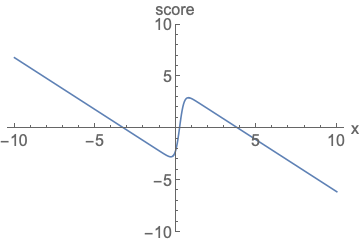
\includegraphics[width=\textwidth]{ScoreFunction.png}
						\caption{\scriptsize Không cần chuẩn hoá.}
					\end{figure}
				\end{column}
			\end{columns}
			
			
			
			\begin{columns}
				\begin{column}{0.5\textwidth}
					\centering
					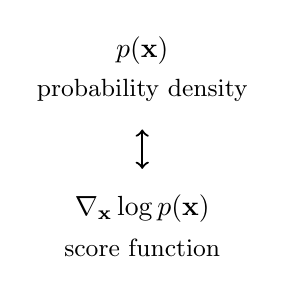
\begin{tikzpicture}
						\node at (0, 1) {$p(\mathbf{x})$};
						
						\node at (0, 0.5) {\small \text{probability density}};
						
						\draw[<->, thick] (0, 0) -- (0, -0.5);
						
						\node at (0, -1) {$\nabla_\mathbf{x} \log p(\mathbf{x})$};
						
						\node at (0, -1.5) {\small \text{score function}};
					\end{tikzpicture}
					
				\end{column}
				\begin{column}{0.5\textwidth}
					\begin{figure}
						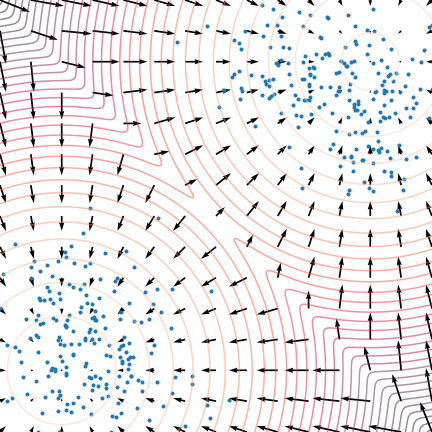
\includegraphics[width=\textwidth]{CompareScoreFunction.png}
						\caption{\scriptsize score function vs probability density}
					\end{figure}
				\end{column}
			\end{columns}
		\end{column}
	\end{columns}	
\end{frame}




%	Ta gọi $\epsilon = \mathcal{N}(0, I)$
%\begin{columns}
%\begin{column}{0.8\textwidth}
%\begin{figure}
%	\centering
%	\includegraphics[width=\textwidth]{OverviewDiffusion}
%\end{figure}
%\end{column}
%
%\begin{column}{0.2\textwidth}
%
%\end{column}
%\end{columns}
%\\
%q(\mathbf{x}_t \vert \mathbf{x}_{t-1}) &= \mathcal{N}(\mathbf{x}_t; \sqrt{\alpha_t} \mathbf{x}_{t-1}, (1 - \alpha_t)\mathbf{I}) \\ 
%\rightarrow q(\mathbf{x}_t \vert \mathbf{x}_0) &= \mathcal{N}(\mathbf{x}_t; \sqrt{\bar{\alpha}_t} \mathbf{x}_0, (1 - \bar{\alpha}_t)\mathbf{I})
